\documentclass[a4paper,11pt]{article}
\usepackage[utf8]{inputenc}
\usepackage[brazilian]{babel}
\usepackage{geometry}
\geometry{margin=0.7in, top=0.9in, bottom=0.8in}
\usepackage{xcolor}
\usepackage{paracol}
\usepackage{titlesec}
\usepackage{enumitem}
\usepackage{fontawesome5}
\usepackage[hidelinks]{hyperref}
\usepackage{lmodern}
\usepackage{graphicx}

\definecolor{primary}{RGB}{13,71,161}
\definecolor{accent}{RGB}{0,150,136}
\definecolor{graytxt}{RGB}{60,60,60}

\hypersetup{
    colorlinks=true,
    linkcolor=primary,
    urlcolor=primary
}

\setcolumnwidth{0.34\textwidth,0.62\textwidth}
\setlist[itemize]{noitemsep, leftmargin=*, label=\textbullet}

\titleformat{\section}
  {\large\bfseries\color{primary}}
  {}{0em}{\MakeUppercase}
  [\color{accent}\titlerule]

\titleformat{\subsection}
  {\normalsize\bfseries\color{accent}}
  {}{0em}{}

\newcommand{\sectionleft}[1]{\subsection*{#1}}
\newcommand{\sectionright}[1]{\section*{#1}}

\setlength{\parindent}{0pt}

\begin{document}

\begin{center}
    {\LARGE\bfseries\color{primary} Fernando Anselmo}\\[2mm]
    {\large\color{graytxt} Technical Full Stack Leader | Solution Architect | Professor}\\[4mm]
    \begin{tabular}{@{}l@{}}
        \faIcon{map-marker} Brasília - DF, Brazil \quad
        \faIcon{envelope} \href{mailto:fernando.anselmo74@gmail.com}{fernando.anselmo74@gmail.com} \\
        \faIcon{phone} (61) 99874-0763 \quad
        \faIcon{linkedin} \href{https://www.linkedin.com/in/fernando-anselmo-bb423623/}{LinkedIn} \quad
        \faIcon{github} \href{https://github.com/fernandoans}{GitHub}
    \end{tabular}
\end{center}
\vspace{2pt}

\section*{Professional Summary}
Strategic technical leader with over 35 years of experience in critical high-performance projects. Specialized in turning technical complexity into clear and efficient solutions with concrete and sustainable results. Author of 18 books, speaker and professor. Specialist in legacy modernization, CI/CD, corporate integrations and Hexagonal and Microservices architectures.
\vspace{2pt}

\begin{paracol}{2}

\sectionleft{Core Competencies}
\begin{itemize}
    \item Java, Spring Boot
    \item Quarkus
    \item J2EE, Struts
    \item Angular 17/21, TypeScript
    \item Node.js, React, React.Native
    \item Docker, Jenkins, Azure DevOps
    \item GitLab CI
    \item PostgreSQL, Oracle, SQL Server
    \item MongoDB, Cassandra, Neo4J
    \item AWS, Oracle Cloud
    \item Hexagonal Architecture
    \item Microservices, DevSecOps
\end{itemize}

\vspace{4pt}
\sectionleft{Certifications}
\begin{itemize}
    \item \textbf{Java Champion – Oracle}
    \item Certified AI Foundations Associate
    \item Certified Programmer Java
    \item Certified Web Developer Java
    \item SCRUM Foundation
\end{itemize}

\vspace{4pt}
\sectionleft{Languages}
\begin{itemize}
    \item English – speaking, reading and writing
    \item Spanish – speaking, reading and writing
\end{itemize}

\switchcolumn

\sectionright{Professional Experience}

\textbf{Senior FullStack Developer – First Decision} \\
\textit{Ministry of Transport / Mauá FalaBr}
\hfill Jan/2025 – present
\begin{itemize}
    \item Angular 17/21 + Java Spring Boot Hexagonal Ports and Adapters
    \item Environment structuring with network segmentation and security
    \item Integrations with PostgreSQL, SQL Server, Oracle and microservices
    \item Architectural support with AI in Node.js/TypeScript
\end{itemize}

\textbf{Senior FullStack Developer – Qintess} \\
\textit{Ministry of Transport}
\hfill Aug/2024 – Jan/2025
\begin{itemize}
    \item Java/Angular with Hexagonal architecture
    \item Git governance, REST APIs
\end{itemize}

\textbf{Java Backend Developer – SEA Tecnologia} \\
\textit{PesqBrasil / Portal SESC}
\hfill Nov/2024 – Mar/2025
\begin{itemize}
    \item Liferay Java, DevSecOps, observability
    \item CI/CD pipelines, capacity planning, high availability
\end{itemize}

\textbf{Systems Analyst IV – CNI/SESI} \hfill Nov/2021 – Oct/2024
\begin{itemize}
    \item Legacy Java refactoring, APIs, Jasper Reports, AD
    \item OutSystems, Power Apps/Power Automate
    \item Kubernetes, GitLab CI/Jenkins, DevSecOps
\end{itemize}

\textbf{Solution Architect – Bancorbrás} \hfill Feb/2021 – Nov/2021
\begin{itemize}
    \item Spring Boot, Quarkus/GraalVM, CI Docker/Jenkins/SonarQube
    \item Stored Procedures modernization, Protheus/AD integration
\end{itemize}

\textbf{Backend Developer – Mirante Tecnologia} \hfill Oct/2019 – Feb/2021
\begin{itemize}
    \item Spring Boot microservices, Jenkins/Docker
    \item Oracle Cloud, TDD, corporate integrations
\end{itemize}

\textbf{Previous Work} \hfill 1987 – Oct/2019
\begin{itemize}
	\item See my LinkedIn for full list
	\item \href{https://www.linkedin.com/in/fernando-anselmo-bb423623/}{Access LinkedIn}
\end{itemize}

\end{paracol}

\section*{Teaching Experience}
\textbf{Computer Science Professor -- UDF - Cruzeiro do Sul Group} \hfill Feb/2023 – present\\
Information Technology Degree – Algorithms, OOP, Mobile, Web, Backend and Mobile.

\textbf{Data Science Professor -- IESB} \hfill Aug/2018 – present\\
Undergraduate/Postgraduate – Python, Hadoop, Java, Mobile, Robotics and Automation.

\vspace{4pt}

\section*{Education}
\begin{itemize}
	\item Postgraduate in Teaching in Information Systems - Faculdade Iguaçu - Ongoing
	\item Postgraduate in Software Architecture - Faculdade Iguaçu - Ongoing
	\item MBA in Information Management - Faculdade Iguaçu - Ongoing
	\item MBA in Technology for Business: Data Science and Big Data - Faculdade Iguaçu - Ongoing
	\item Postgraduate in proficiency in digital technologies for entrepreneurial education - Secretaria de Educação GDF / SEBRAE - Ongoing
	\item Postgraduate in Applied Statistics - Faculdade Anhanguera - 2020
	\item Technical Degree in Digital Games - IFB - 2019
	\item Postgraduate in Advanced Business Management - Faculdade JK - 2016
	\item Bachelor in Information Technology Management - FacSenac - 2011
	\item Specialization in Programming - Faculdades Integradas da Católica - 1996
\end{itemize}

\section*{Competency Map}
\begin{center}
    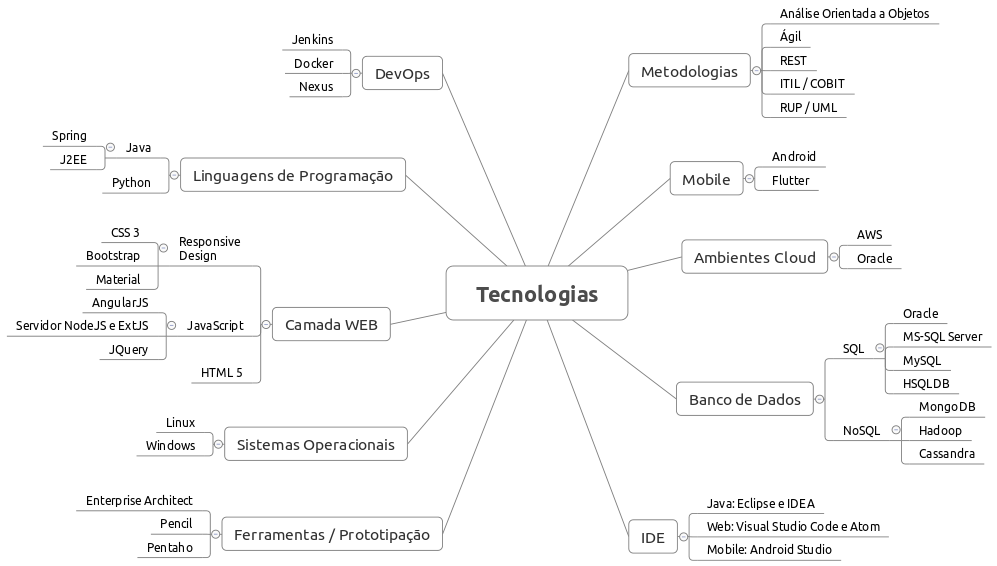
\includegraphics[width=0.95\textwidth]{imagens/tecnologias.png}
\end{center}

\end{document}
